\emph{Cancer} is an umbrella term for a group of diseases caused by abnormal cell growth in different parts of the body. The accumulation of extra cells usually forms a mass of tissue called a \emph{tumor}. Tumors can be benign or malignant: \emph{benign tumors} are noncancerous, lack the ability to invade surrounding tissue and will not regrow if removed from the body;  malignant or \emph{cancerous tumors} are harmful, can invade nearby organs and tissues (\emph{invasive cancer}), can spread to other parts of the body (\emph{metastasis}) and will sometimes regrow when removed~\cite{NCI2012}.

\emph{Breast cancer} forms in tissues of the breast. The two most common types of breast cancer are \emph{ductal carcinoma} and \emph{lobular carcinoma}, which start in the breast ducts and lobules, respectively (Fig.~\ref{fig:BreastAnatomy}). Breast cancer \emph{incidence rate}, the number of new cases in a specified population during a year, is the highest of any cancer among American women. Its \emph{mortality rate}, the number of deaths during a year, is also one of the highest of any cancer~\cite{Howlader2014}.

\begin{figure}[h]
	\centering
	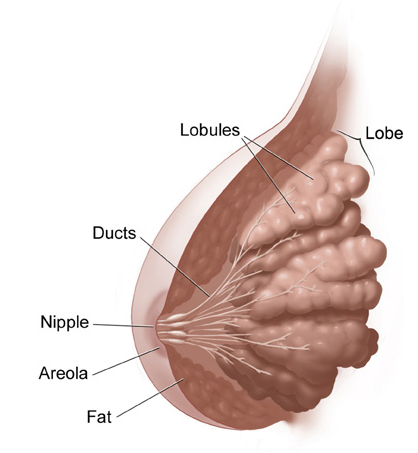
\includegraphics[width = 0.34\textwidth]{plots/breastAnatomy.png}
	\caption[Anatomy of the female breast]{Anatomy of the female breast. Image courtesy of~\cite{NCI2012}.}
	\label{fig:BreastAnatomy}
\end{figure}

The \emph{cancer stage} depends on the size of the tumor and whether the cancer cells have spread to neighboring tissue or other parts of the body. It is expressed as a Roman numeral ranging from 0 through IV; stage I cancer is considered \emph{early-stage breast cancer} and stage IV cancer is considered \emph{advanced}. Stage 0 describes non-invasive breast cancers, also known as \emph{carcinoma in situ}. Stage I, II and III describe invasive breast cancer, i.e., cancer has invaded normal, surrounding breast tissue. Stage IV is used to describe metastatic cancer, i.e., it has spread beyond nearby tissue to other organs of the body.

\subsection{Mammograms}
%\subsubsection{Mammograms}
A \emph{mammogram} is an x-ray image of the breast. Radiologists use \emph{screening mammograms} (normally composed of two mammograms of each breast) to check for breast cancer signs on women who lack symptoms of the disease. If an abnormality is found, a \emph{diagnostic mammogram} is ordered; these are detailed x-ray pictures of the suspicious region~\cite{NCI2014}. A standard mammogram is shown in Figure~\ref{fig:normalMammogram}.

\begin{figure}[h]
	\centering
	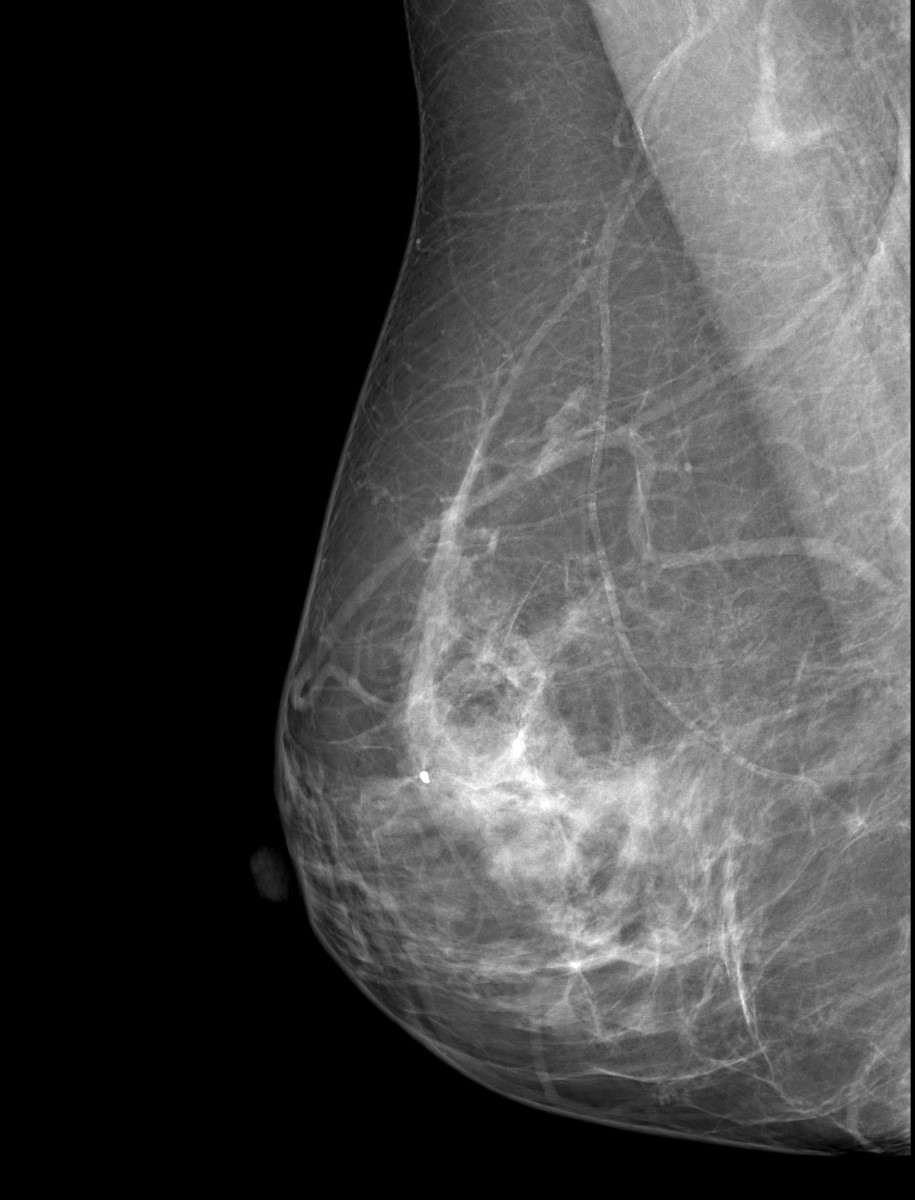
\includegraphics[width = 0.25\textwidth]{plots/normalMammogram.jpg}
	\caption[A digital mammogram]{A standard mammogram.}
	\label{fig:normalMammogram}
\end{figure}

Having a screening mammogram in a regular basis is the most effective method for detecting breast cancer early; around 85\% of breast cancers can be detected in a screening mammogram~\cite{BCSC2013}. Nevertheless, screening mammograms have many limitations: a high false positive rate, overtreatment in Stage 0 cancer, false negative results for women with high breast density, radiation exposure and physical and psychological discomfort~\cite{NCI2014}.

Radiologists look primarily for microcalcifications and breast masses. \emph{Microcalcifications} are tiny deposits of calcium in the breast tissue that can be a sign of early breast cancer if found in clusters with irregular layout and shapes (Fig.~\ref{fig:breastCancerSigns}). \emph{Breast masses} or breast lumps are a variety of things: fluid-filled cysts, fibric tissues, noncancerous or cancerous tumors, among others. A mass can be a sign of breast cancer if it has an irregular shape and poorly defined margins (Fig.~\ref{fig:breastCancerSigns}). Radiologists will also consider the breast density of the patient when reading a mammogram given that high breast density is linked to a higher risk of breast cancer~\cite{ACS2014}.
\begin{comment} My classification
Lesion
	Mass = Lump(This is palpable)
		Malignant = Cancerous
			Tumors
		Benign = Noncancerous
			Tumors
			Cysts
			Fibrosis/Fibroadenoma
	Microcalcifications (benign or malignant)

Tumors are abnormal growths of cells, cysts ae filled with fluid and fibrosis are "firmness in the connective tissues". Lesion is anything suspicious in a mammogram
Detection: Find lesions (malignant or benign)
Diagnosis: Find malignant lesions
\end{comment}

\begin{figure}[h]
	\centering
	\begin{subfigure}{0.24\textwidth}
                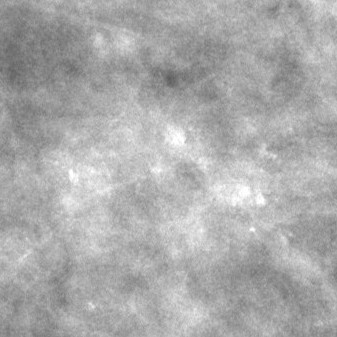
\includegraphics[width=\textwidth]{plots/breastMicrocalcification.jpg}
        \end{subfigure}
	~
	\begin{subfigure}{0.24\textwidth}
                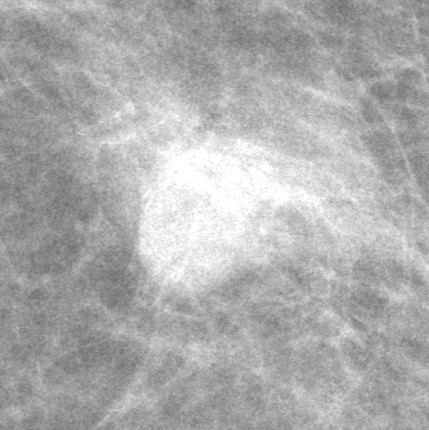
\includegraphics[width=\textwidth]{plots/breastMass.jpg}
        \end{subfigure}
	\caption[Signs of possible breast cancer]{Signs of possible breast cancer in a mammogram. Left: A cluster of microcalcifications in an irregular layout. Right: A poorly defined breast mass.}
	\label{fig:breastCancerSigns}
\end{figure}

%Conventional mammography uses film to record x-ray images of the breast. \emph{Digital mammography}, on the other hand, uses digital receptors that convert x-rays into electrical signals and stores the image electronically. 
Conventional mammography records mammograms in film; \emph{digital mammography}, on the other hand, converts x-rays into electrical signals and stores images electronically.
Digital mammograms offer a clearer picture of the breast and ease manipulation and sharing between health care providers.
% However, researchers still debate whether [[its|their] use over| they] [surpass| improve on|outperform|[offers|have] an advantage over|are more effective than|benefit] film mammograms [in|for] [identifying breast cancer|breast cancer detection].
Although researchers still debate whether they offer an advantage over film mammograms~\cite{Kerlikowske2011, Pisano2008, Skaane2007}, digital mammography has become standard in breast cancer screening. Figure~\ref{fig:normalMammogram} is, in fact, a digital mammogram.
\emph{Digital tomosynthesis} is a new technology that produces three-dimensional x-ray images of the breast and improves the efficacy of mammograms in certain escenarios~\cite{Tagliafico2016}.%http://jco.ascopubs.org/content/early/2016/03/07/JCO.2015.63.4147.abstract
%is expected to improve the efficacy of mammograms. Studies comparing the two techniques have not yet been published~\cite{NCI2014}.

\emph{Computer-aided detection (CAD)} systems assist radiologists during screening signaling suspicious areas and displaying relevant information. Detection or CADe looks for any type of lesion while diagnosis or CADx focuses on malignant lesions. Whether their use improves accuracy has been challenged~\cite{Lehman2015}.

% option: Delete this, downgrade mammograms to subsubsection and add the bcdr info in the solution/data set/database part. Maybe also leave the first paragraph in here as part of mammograms subsection, only change it to say "Mammography databases are important"
% option: do not add anything
\subsection{Mammographic databases}
%Databases are essential to mammographic image analysis;
%annotated
Researchers use data from previous patients---mammograms, segmentations and clinical features\textemdash to train and evaluate their models. 
%Databases offer pixel-wise labelled mammograms, lesions are segmented by expert radiologists.
%For this purpose, lesions are manually segmented to produce pixel-wise labels.
\emph{Contrast resolution}, the number of gray values per pixel, and \emph{spatial resolution}, breast area per pixel, dictate the quality of a digital mammogram: 12-bit images ($2^{12} = 4048$ gray values) with pixel size of at most 0.1mm are prefered. Many publicly available databases, including those described below, satisfy these conditions.

The Digital Database for Screening Mammography (DDSM)~\cite{Heath2001} is the most popular database used for CAD development. It is composed of around 10.5K digitized film mammograms from 2620 patients. Mammograms are either 12-bit or 16-bit images with 0.05 mm spatial resolution. Lesion segmentations are provided along with its type, assesment, subtlety and malignancy.%Patient data is also provided.
%Type is mass, microcalcification, assesment (1-5) in BIRADs, subtlety(1-5) and 

The BancoWeb database~\cite{Nepomuceno2011} consists of around 1.5K digitized film mammograms from 300 Brazilian patients. Mammograms are 12-bit images with 0.075 or 0.15 mm pixel size. Although few lesions are segmented, this repository may be useful to assess performance in Latin American patients. Its current state is unknown.

Lastly, the Breast Cancer Digital Repository (BCDR-DM)~\cite{Moura2013a, Moura2013b} consists of around 1.2K digital mammograms from 237 patients. Mammograms are 8-bit images with 0.07mm spatial resolution.
Lesion segmentations are provided as well as their assesment, hand-crafted texture and shape features and relevant clinical data.
%It provides lesion segmentations and assesments, hand-crafted texture and shape features and relevant clinical data

\begin{comment}
Another small digital mammogram repository is called INbreast~\cite{Moreira2012}. It consists of 410 digital mammograms from 115 patients. Each mammogram is a 14-bit image with 0.7 mm spatial resolution. Lesion boundaries are accurately marked and its information is also included. This could be used in conjunction with the BCDR-DM repository.

Finally,~\cite{Zheng2012} used a private repository of around 6.5K digital mammograms obtained from 1120 patients. Specifics of contrast and spatial resolution are not provided but they are most probably good enough. Lesions are marked (with a circle) on the mammograms and lesion and patient information is provided. Even though this is a private repository of the University of Pittsburgh, if needed, we could ask them for access to it. This may not be plausible given the complications of sharing personal (granted anonymized) information and the size of the database.
\end{comment}

This section was written using information from the National Cancer Institute. We recommend to visit its website (\url{www.cancer.gov}) for further details.
